%! TeX root = master.tex
% !TEX program = lualatex
\lecture{7}{31-03-2026}{}{}
\subsection{Kernel function}

When using feature expansion, we realised that we could use any function of the input — but two problems arise:
\begin{itemize}
  \item \textbf{Choice}: how do we choose a good mapping $\phi(\cdot)$?
  \item \textbf{Scalability}: when $\phi(x) \in \mathbb{R}^F$ with $F \gg D$ (or even $F = \infty$), explicitly computing $\phi(x)$ and then $\phi(x_i)^T\phi(x_j)$ becomes intractable.
\end{itemize}
Kernel functions solve both problems at once.

Many machine learning algorithms rely on the \textbf{dot product} between inputs:
\[
x_i^T x_j
\]
This quantity is proportional to the cosine of the angle between the vectors, thus encoding a notion of \textbf{similarity}.

When performing \textbf{feature expansion}, inputs are mapped through a function $\phi(\cdot)$, leading to:
\[
\phi(x_i)^T \phi(x_j)
\]
which defines a new similarity measure in the transformed feature space.

Instead of explicitly computing $\phi(\cdot)$, one can define a function:
$
k(x_i, x_j)
$
called a \textbf{kernel function}, such that:
\[
k(x_i, x_j) = \phi(x_i)^T \phi(x_j) = \left\|\phi(x)\right\|^2 
\]
The mapping $\phi(\cdot)$ may be unknown or computationally expensive, but the kernel function allows us to compute similarities implicitly.

\subsubsection{Example}
\textbf{Polynomial kernel}
\[
  k(x_i,x_j) = (x_i^T x_j + c)^d
\]
has two hyper-parameters: The bias $c$, the degree of the polynomial $d$. 

His corresponding mappings $\phi(\cdot)$ for $c = 1$ and $d = 2$ is \[
  \phi(x) = [\ (x^{(1)})^2,(x^{(2)})^2,\sqrt{2} x^{(1)}x^{(2)}, \sqrt{2}x^{(1)}, \sqrt{2}x^{(2)}, 1]\
\]
And corresponds to the quadratic kernel \[
  k(x_i, x_j) = (x_i^T x_j + 1)^2
\]
Note that computing the kernel value only requires 3 multiplications,
versus 6 when computing the dot product $\phi(x_i)^T \phi(x_j)$.

\textbf{Gaussian kernel}
\[
  k(x_i, x_j) = \exp(- \frac{\left\|x_i - x_j\right\|^2}{2 \sigma ^2})
\]
Hyper-parameter : the bandwith $\sigma$. 

But for this kernel there is no explicit mapping $\phi(\cdot)$ (in theory, this kernel corresponds to a mapping to an infinite dimensional space).

$Visualization$: 

2D inputs, one sample $x_j = \[5,3\]^T$, and vary $x_i$


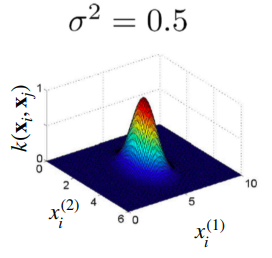
\includegraphics[width=0.33\linewidth]{images/img_20260402_135010.png}
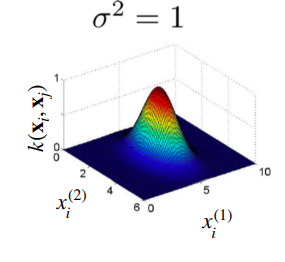
\includegraphics[width=0.33\linewidth]{images/img_20260402_135030.png}
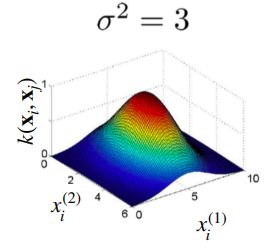
\includegraphics[width=0.33\linewidth]{images/img_20260402_135046.png}

\subsubsection{Trick}
Since a kernel function corresponds to a similarity, as a dot
product, one can replace any dot product between two
samples in the solution of an ML algorithm with a kernel
function \to $kernelizing$ an algorithm (not only for linear model !).

\subsubsection{Kernelization: Notation}
The kernel function computes a similarity between two samples, and can be written as $k(x_i, x_j)$. 

We could to use the kernel function to encode the similarity between one sample and all traning samples (matrix $X$): 
\[
  k(X, x_i) = \begin{pmatrix} k(x_1, x_j) \\ k(x_2, x_j) \\ \vdots \\ k(x_N, x_j)    
  \end{pmatrix} \in \mathbb{R}^N
\]

Furthermore, we can define the \textbf{kernel matrix}, a squared matrix, which each entry $(i,j)$ contains the kernel function evaluate between training sample $i$ and training sample $j$ \[
  K = \begin{pmatrix}
    k(x_1, x_1) & k(x_1, x_2) & \cdots & k(x_1, x_N) \\
    k(x_2, x_1) & k(x_2, x_2) & \cdots & k(x_2, x_N) \\
    \vdots & \vdots & \vdots & \vdots \\
    k(x_N, x_1) & k(x_N, x_2) & \cdots & k(x_N, x_N)
  \end{pmatrix} \in \mathbb{R}^{N \times N}
\]

\subsubsection{Kernel regression}
To kernelize linear regression we need to rewrite the solution so that $\phi(\cdot)$ only appears inside dot products — which we can then replace by $k(\cdot,\cdot)$, to do so we can make use of the Representer theorem (useful too to kernelize other algorithms). 

\textbf{Representer theorem}

\begin{itemize}
  \item Main Idea: Optimal solutions exist within a finite linear combination of training data 
  \item Goal: Reduce infinite-dimensional problems to finite-dimensional ones
\end{itemize} 

In essence, this theorem states that the minimizer of a
regularized empirical risk function can be represented as a
linear combination of the points in the high dimensional
space.That is, we can write
\[
  w^* = \sum_{i=1}^{N}\alpha_i^* \phi(x_i) = \Phi^T \alpha^*
\]

So instead of searching for a minimizer of the empirical risk in
terms of \textbf{w}, we search for one in terms of new variables $\{ \alpha _i \}$

Therefore, the empirical risk : \[
  R(w) = \sum_{i=1}^{N}(w^T \phi(x_i) - y_i)^2 
\]
is re-written as 
\[
  R(\alpha) = \sum_{i=1}^{N}(\alpha ^T \Phi \phi (x_i) - y_i)^2 = \sum_{i=1}^{N} (\alpha ^T k(X, x_i) - y_i)^2 
\] (as $\Phi \cdot \phi(x_i)$ is the dot product of all training samples and sample i !)

The gradient of the risk w.r.t $\alpha$ is given by \[
  \nabla R(\alpha) = 2 \sum_{i=1}^{N} k(X,x_i)(k(X,x_i)^T \alpha - y_i) = 2KK \alpha - 2 Ky
\] with \textbf{K} the $N \times N$ training kernel matrix, obtained by evaluating the kernel function between all pairs of training samples. 

Setting the gradient to 0 yields \[
  2KK \alpha^* = 2Ky \iff Ka^* = y
\]which gives the solution \[
\alpha ^* = (K)^{-1} y
\] 

Putting this solution back in the definition of $w^*$ gives us \[
  w^* = \Phi^T(K)^{-1}y
\]

This solution still depends on $\Phi$, which we argued could be unknown. 

Therefore the prediction for a new sample \textbf{x} is given by :\[
  \hat{y} = (w^*)^T \phi(x) = y^T (K)^{-1} \Phi \phi(x) = y^T (K)^{-1}k(X,x)
\]

Note that the quantity $y^T (K)^{-1}$ only depends on the training
data, and thus can be pre-computed and reuse for every test sample. 

\subsubsection{Kernel ridge regression}
Using the Representer theorem, the regularized empirical risk \[
  E(w) = \sum_{i=1}^{N} (w^T \phi(x_i) - y_i)^2 + \lambda w^Tw
\]
Can be re-written as \[
  E(\alpha) = \sum_{i=1}^{N} (\alpha ^T \Phi \phi(x_i) - y_i)^2 + \lambda \alpha ^T \Phi \Phi ^T \alpha =  \sum_{i=1}^{N} (\alpha ^T k(X, x_i) - y_i)^2 + \lambda \alpha ^T K \alpha 
\]
The gradient become \[
  \nabla _a E(\alpha) = 2K (K+ \lambda I_N)\alpha - 2Ky
\]Setting it to zero yields the solution \[
\alpha ^* = (K + \lambda I_N)^{-1}y
\]

\subsubsection{Kernel ridge regression with multiple outputs}

To handle nonlinear problems, we can then again work in a
different feature space $\phi (\cdot)$ and write the regularized
empirical risk
\[
  E(W) = \sum_{i=1}^{N} \left\|W^T \phi(x_i) - y_i\right\|^2 + \lambda \left\|W\right\|_F^2
\]
And by using the Representer theorem, we can again derive a solution that depend on kernel values $k(x_i, x_j$ instead of $\phi(\cdot)$. 

The solution is given by \[
  W^* = \Phi ^T (K + \lambda I)^{-1} Y 
\]where \Phi is the same matrix concatenating the training inputs $\{ \phi(x_i) \}$, and $Y \in \mathbb{R}^{N \times C}$ is the matrix stacking the training output vectors. 

The prediction vector for a test sample is given as \[
  \hat{y} = (W^*)^T \phi(x) = Y^T (K + \lambda I)^{-1} \Phi \phi(x) = Y^T (K + \lambda I)^{-1} k(X,x)
\]
\subsubsection{Remark}
As the results of kernel ridge regression strongly depend on the choice of kernel and of the hyperparameter values for a given kernel, it may be natural to ask ourself how to find good parameters. 

The answer is by \textbf{cross-validation}. Each kernel and each hyperparameter value
corresponds to a different model. We can then separate our training
data into training and validation sets, train each model with the new
training data, and choose the one that performs the best on the
validation data

\subsubsection{Advantages and Drawbacks of kernel methods}
\textbf{Advantages:} 
\begin{itemize}
  \item Can effectively handle nonlinearly-separable data
  \item Often have nice solutions (e.g., closed-form, convex)
\end{itemize}

\textbf{Drawbacks:}
\begin{itemize}
  \item Depend on the choice of kernel and hyper-parameter(s)
  \item Computational complexity depends on the number of samples. 
  \begin{itemize}
    \item E.g., for kernel ridge regression, one needs to invert an $N \times N$ matrix, which
requires $O(N^3)$ operations
  \end{itemize}
\end{itemize}
